

\section{评估}
\label{sec:evaluation}

% \subsection{Evaluation of Base Models}

如前所述，GLM-5 标志着从 vibe coding 向 agentic engineering 新时代的过渡。
我们首先在智能体、推理与编码（ARC）基准上，将 GLM-5 与前沿模型进行评测。
为全面评估 GLM-5 在真实智能体工程场景中的表现，我们提出新的内部评测套件 CC-Bench-V2，覆盖前端、后端与长时程任务。
最后，我们在五类常见真实场景中评估 GLM-5 的通用能力。


\subsection{ARC 基准评估}

我们在表~\ref{tab:eval_arc} 中报告 ARC 基准主要结果，对比 GLM-5 与 GLM-4.7、DeepSeek-V3.2~\cite{liu2025deepseek}、Kimi-K2.5~\cite{team2026kimi}、Claude Opus 4.5~\cite{opus4.5}、Gemini 3 Pro~\cite{gemini3} 以及 GPT-5.2（xhigh）~\cite{gpt-5.2}。
总体而言，GLM-5 相较 GLM-4.7 实现显著提升，并在开源模型中达到最先进性能，缩小了与 Claude Opus 4.5 等闭源模型的差距。评测细节见第~\ref{sec:eval_details_arc} 节。

\begin{table}[htbp]
\centering
\caption{\label{tab:eval_arc} GLM-5 与开源/闭源模型对比。标记 * 的结果来自 HLE 全量集合。标记 $^\dagger$ 的结果在经过核验的 Terminal-Bench 2.0 上评估，修复了部分歧义指令。GDPval-AA Elo 记录于 2026 年 2 月 15 日。每个基准最高分以 \textbf{粗体} 标注，第二高分以下划线 \underline{标注}。}
\setlength{\tabcolsep}{3pt}
\renewcommand{\arraystretch}{1.15}
\begin{tabular}{lccccccc}
\toprule
& \textbf{GLM-5} & \textbf{GLM-4.7} & \begin{tabular}[c]{@{}c@{}}\textbf{DeepSeek}\\\textbf{-V3.2}\end{tabular} & \begin{tabular}[c]{@{}c@{}}\textbf{Kimi}\\\textbf{K2.5}\end{tabular} & \begin{tabular}[c]{@{}c@{}}\textbf{Claude}\\\textbf{Opus 4.5}\end{tabular} & \begin{tabular}[c]{@{}c@{}}\textbf{Gemini}\\\textbf{3 Pro}\end{tabular} & \begin{tabular}[c]{@{}c@{}}\textbf{GPT-5.2}\\\textbf{(xhigh)}\end{tabular}  \\
\midrule
\textit{Reasoning \& General} & & & & & & & \\
HLE & 30.5 & 24.8 & 25.1 & 31.5 & 28.4 & \textbf{37.2} & \underline{35.4} \\
HLE (w/ Tools) & \underline{50.4} & 42.8 & 40.8 & \textbf{51.8} & 43.4* & 45.8* & 45.5* \\
AIME 2026 I & 92.7 & \underline{92.9} & 92.7 & 92.5 & \textbf{93.3} & 90.6 & - \\

HMMT Feb. 2025 & \underline{97.9} & 97.1 & 92.5 & 95.4 & 92.9 & 97.3 & \textbf{99.4} \\
HMMT Nov. 2025 & \underline{96.9} & 93.5 & 90.2 & 91.1 & 91.7 & 93.0 & \textbf{97.1} \\
IMO-AnswerBench & 82.5 & 82.0 & 78.3 & 81.8 & 78.5 & \underline{83.3} & \textbf{86.3} \\
GPQA-Diamond & 86.0 & 85.7 & 82.4 & 87.6 & 87.0 & \underline{91.9} & \textbf{92.4} \\
LongBench v2 & \underline{64.5} & 59.1 & 59.8 & 61.0 & 64.4 & \textbf{68.2} & 59.8 \\
\midrule
\textit{Coding} & & & & & & & \\
SWE-bench Verified & 77.8 & 73.8 & 73.1 & 76.8 & \textbf{80.9} & 76.2 & \underline{80.0} \\
SWE-bench Multilingual & \underline{73.3} & 66.7 & 70.2 & 73.0 & \textbf{77.5} & 65.0 & 72.0 \\
\begin{tabular}[c]{@{}l@{}}Terminal-Bench 2.0\\{\small \ (Terminus-2)}\end{tabular} & \makecell[c]{\underline{56.2} /\\ 60.7$^\dagger$} & 41.0 & 39.3 & 50.8 & \textbf{59.3} & 54.2 & 54.0 \\
\begin{tabular}[c]{@{}l@{}}Terminal-Bench 2.0\\{\small \ (Claude Code)}\end{tabular} & \makecell[c]{\underline{56.2} /\\ 61.1$^\dagger$} & 32.8 & 46.4 & - & \textbf{57.9} & - & - \\
CyberGym & \underline{43.2} & 23.5 & 17.3 & 41.3 & \textbf{50.6} & 39.9 & - \\
\midrule
\textit{Agentic} & & & & & & & \\
BrowseComp & \textbf{62.0} & 52.0 & 51.4 & \underline{60.6} & 37.0 & 37.8 & - \\
\begin{tabular}[c]{@{}l@{}}BrowseComp\\{\small \ (w/ Context Manage)}\end{tabular} & \textbf{75.9} & 67.5 & 67.6 & \underline{74.9} & 57.8 & 59.2 & 65.8 \\
BrowseComp-ZH & \underline{72.7} & 66.6 & 65.0 & 62.3 & 62.4 & 66.8 & \textbf{76.1} \\
$\tau^2$-Bench & 89.7 & 87.4 & 85.3 & 80.2 & \textbf{91.6} & \underline{90.7} & 85.5 \\
MCP-Atlas (Public Set) & \underline{67.8} & 52.0 & 62.2 & 63.8 & 65.2 & 66.6 & \textbf{68.0} \\
Tool-Decathlon & 39.2 & 23.8 & 35.2 & 27.8 & \underline{43.5} & 36.4 & \textbf{46.3} \\
Vending-Bench 2 & \$4,432 & \$2,377 & \$1,034 & \$1,198 & \underline{\$4,967} & \textbf{\$5,478} & \$3,591 \\
GDPval-AA Elo & \underline{1,409} & 1,198 & 1,195 & 1,288 & 1,400 & 1,201 & \textbf{1,462} \\
\bottomrule
\end{tabular}
\end{table}




\subsubsection{推理与通用基准评估}

% Table~\ref{tab:eval_arc} shows the performance of GLM-5 and other frontier LLMs on 
在推理与通用基准方面，
我们评测了 Humanity’s Last Exam（HLE）~\cite{phan2025humanity}、AIME 2026、HMMT 2025、IMO-AnswerBench~\cite{luong2025towards}、GPQA-Diamond~\cite{rein2024gpqa} 以及 LongBench v2~\cite{bai-etal-2025-longbench}。
对于 HLE，我们仅评测文本子集，并使用 GPT-5.2（medium）作为 judge 模型。多数推理任务采用 131,072 的最大生成长度，而 HLE-with-tools 使用 202,752 最大 tokens。

从表~\ref{tab:eval_arc} 可见，GLM-5 在推理任务上与强开源基线 Kimi-K2.5 表现相当。
与闭源模型相比，GLM-5 在 HLE（with tools）上优于 Claude Opus 4.5 和 Gemini 3 Pro。
相较前代 GLM-4.7，GLM-5 在 HLE（含/不含工具）上均有显著提升。
在 HMMT Feb./Nov. 2025 上，GLM-5 优于 Claude Opus 4.5 与 Gemini 3 Pro。
GLM-5 在长上下文任务上也取得显著进展，在长上下文推理基准 LongBench v2 中取得仅次于 Gemini 3 Pro 的第二高分。


\subsubsection{编码基准评估}

在编码基准方面，我们在 SWE-bench Verified~\cite{jimenez2023swe}、SWE-bench Multilingual~\cite{yang2025swemulti}、Terminal Bench 2.0~\cite{tbench_2025} 与 CyberGym~\cite{wang2025cybergym} 上评测 LLM。
对 SWE-bench Verified \& Multilingual，我们在 OpenHands 框架中使用为 GLM-5 定制的指令提示。
对 Terminal-Bench 2.0，我们采用 Terminus-2 与 Claude Code 两个智能体框架，并额外报告修复部分歧义指令后的 verified Terminal-Bench 2.0 表现\footnote{更多信息见 \url{https://huggingface.co/datasets/zai-org/terminal-bench-2-verified}}。
CyberGym 在 Claude Code 2.1.18 中评测。

从表~\ref{tab:eval_arc} 可见，GLM-5 在开源 LLM 中于编码基准上达到 SOTA。
与闭源 LLM 相比，GLM-5 在 SWE-bench Verified 上优于 Gemini 3 Pro，在 SWE-bench Multilingual 上也优于 Gemini 3 Pro 与 GPT-5.2（xhigh）。
在 Terminal-Bench 2.0 上，GLM-5 与 Claude Opus 4.5 结果相当，并在修复歧义指令后表现更优。
为展示编码能力泛化性，我们在两个智能体框架上评测 Terminal Bench 2.0，GLM-5 在两者上均表现稳定。
在网络安全编码基准（CyberGym）上，GLM-5 相比 GLM-4.7 显著提升，仅次于 Claude Opus 4.5。


\subsubsection{智能体能力评估}


在智能体基准方面，我们评测了 GLM-5 与前沿模型在 BrowseComp~\cite{wei2025browsecomp}、BrowseComp-ZH~\cite{zhou2025browsecompzh}、$\tau^2$-Bench~\cite{barres2025tau2}、MCP-Atlas~\cite{bandi2026mcp}、Tool-Decathlon~\cite{li2025tool}、Vending-Bench 2~\cite{backlund2025vending} 与 GDPval-AA~\cite{patwardhan2025gdpval} 上的表现。
% BC context manage?
BrowseComp 衡量语言智能体通过网页浏览解决挑战性问题的能力，BrowseComp-ZH 主要面向中文网页。
我们在 BrowseComp 中使用 discard-all 作为上下文管理策略，与 DeepSeek-V3.2 和 Kimi K2.5 一致。
$\tau^2$-Bench 评估对话智能体在双控制环境中的能力。我们对 Retail 与 Telecom 加入小幅提示调整，以避免过早用户终止导致失败（见 \ref{sec:tau_user_prompt}）。对 Airline，我们应用 Claude Opus 4.5 system card~\cite{opus4.5} 中提出的领域修复以获得更准确结果。
MCP-Atlas 是真实工具使用基准，在给定 Model Context Protocol（MCP）服务器条件下评估 LLM 在多步工作流中的表现。为公平对比，我们在 500 任务公开集上重评全部模型，并将单任务超时从 4 分钟扩展到 10 分钟，以避免部署条件导致任务失败。MCP-Atlas 使用 Gemini 3 Pro 作为 judge。
Tool-Decathlon 同样是工具使用基准，但面向真实长时程任务。
Vending-Bench 2 在模拟环境中衡量 LLM 在长时间跨度商业场景中的智能体能力，相比前代 Vending-Bench 引入更多真实因素。
GDPval 聚焦 AI 智能体在具有经济价值任务上的表现。

从表~\ref{tab:eval_arc} 可见，GLM-5 在智能体基准上相较 GLM-4.7 显著提升。
在 BrowseComp（含/不含上下文管理）上，GLM-5 在前沿 LLM 中达到 SOTA。
在 BrowseComp-ZH 上，GLM-5 也优于 Claude Opus 4.5 与 Gemini 3 Pro。
在三项工具使用智能体任务（$\tau^2$-Bench、MCP-Atlas、Tool-Decathlon）上，GLM-5 与 Claude Opus 4.5 表现相当，显示出 GLM-5 的强工具使用能力。
GLM-5 在 Vending-Bench 2 上的结果（\$4,432）进一步证明其商业任务长时程能力。
在经济场景中，GLM-5 在 GDPval-AA 上优于 Claude Opus 4.5，仅次于 GPT-5.2（xhigh）。


\subsection{真实智能体工程体验评估}

真实体验比榜单更重要。我们将内部 CC-Bench 升级为 CC-Bench-V2，用于评估模型在真实智能体工程环境中能否正确完成前端、后端与长时程端到端任务。CC-Bench-V2 完全去除人工标注，基于 Claude Code 与其他 agent harness，结合单元测试和 Agent-as-a-Judge 技术实现全自动评估。

\textbf{前端。} 我们先构建智能体生成的前端项目，并检查语法、依赖与兼容性错误。随后使用 Agent-as-a-Judge，通过配备 Playwright 与 bash 工具的 GUI 智能体模拟用户交互，验证端到端正确性。

\textbf{后端。} 任务来自真实开源项目，覆盖 C++、Rust、Go、Java、TypeScript、Python，包含功能实现、缺陷修复、回归修复与性能优化。每次改动都必须在真实工程约束下通过完整单元测试。

\textbf{长时程。} 我们先评估模型在大型代码库中的信息检索能力，这是像人类开发者一样定位文件、理解项目上下文的前提。随后通过多步链式任务评估端到端正确性：我们挖掘已合并 PR 及其大量提交历史，并将提交聚类成连贯任务链。智能体按顺序执行这些任务链，以测试其跨阶段保持上下文与处理依赖关系的能力。评估结合单元测试与 Agent-as-a-Judge，同时验证功能正确性与语义一致性。

\begin{table}[h!]
\centering
\caption{CC-Bench-V2 在前端、后端与长时程任务上的评测结果。\textbf{BSR}：构建成功率；\textbf{ISR}：实例成功率；\textbf{CSR}：检查项成功率。}
\label{tab:cc-bench-v2}
\begin{tabular}{llcccc}
\toprule
\textbf{Category} & \textbf{Task} & \textbf{Metric} & \textbf{GLM-5} & \textbf{GLM-4.7} & \textbf{Claude Opus 4.5} \\
\midrule
\multirow{6}{*}{Frontend}
  & HTML           & ISR     & 38.9          & 35.4          & \textbf{52.2} \\
  &                & CSR     & 76.3          & 64.9          & \textbf{82.2} \\[2pt]
  & React          & ISR     & 34.6          & 17.2          & \textbf{39.7} \\
  &                & CSR     & \textbf{71.0} & 49.4          & 70.7          \\[2pt]
  & Vue            & ISR     & 32.7          & 24.5          & \textbf{46.9} \\
  &                & CSR     & \textbf{77.1} & 53.8          & 74.3          \\
\midrule
\multirow{4}{*}{Build}
  & React          & BSR     & \textbf{100}  & 65.0          & 95.0          \\
  & Vue            & BSR     & \textbf{100}  & 70.0          & \textbf{100}  \\
  & Svelte         & BSR     & \textbf{100}  & 60.0          & 90.0          \\
  & Next.js        & BSR     & 95.0          & 70.0          & 80.0          \\
\midrule
Backend            & Engineering & Pass@1  & 25.8          & 19.6          & \textbf{26.9} \\
\midrule
\multirow{2}{*}{Long-horizon}
  & Repo Exploration   & Pass@1  & \textbf{65.6} & 47.8          & 64.5          \\
  & Chained Tasks      & Pass@1  & 52.3          & 43.0          & \textbf{61.6} \\
\bottomrule
\end{tabular}
\end{table}



\subsubsection{前端评估——Agent-as-a-Judge}

我们开发了面向前端开发场景的综合自动化评测基准。该基准覆盖开发者常见应用类型，包括落地页、管理看板、数据可视化、图形与动画、在线生产力工具、交互游戏、表单驱动工作流等，技术栈覆盖 HTML、React、Vue、Svelte 与 Next.js。

每个测试样例由包含多个可实现规格的 \textit{Task} 与对应 \textit{Checklist} 组成，后者的每个 check-item 都直接来源于规格要求。
评估流程采用两阶段：1）\textbf{静态验证}：先验证生成代码是否可成功构建与运行。2）\textbf{Agent-as-a-Judge}：对可运行代码，使用 GUI 智能体模拟人工测试，交互式验证每个检查项并按需求完成度评分。
我们定义以下指标：\textit{Build Success Rate（BSR）} 衡量可成功初始化并运行的项目比例；\textit{Instance Success Rate（ISR）} 衡量通过全部规格要求的项目比例；\textit{Check-item Success Rate（CSR）} 衡量全部检查项上的细粒度完成率。
数据分布、构建与验证流程细节见附录~\ref{sec:frontend_eval_data_cons}。

\begin{figure}[h!]
    \centering
    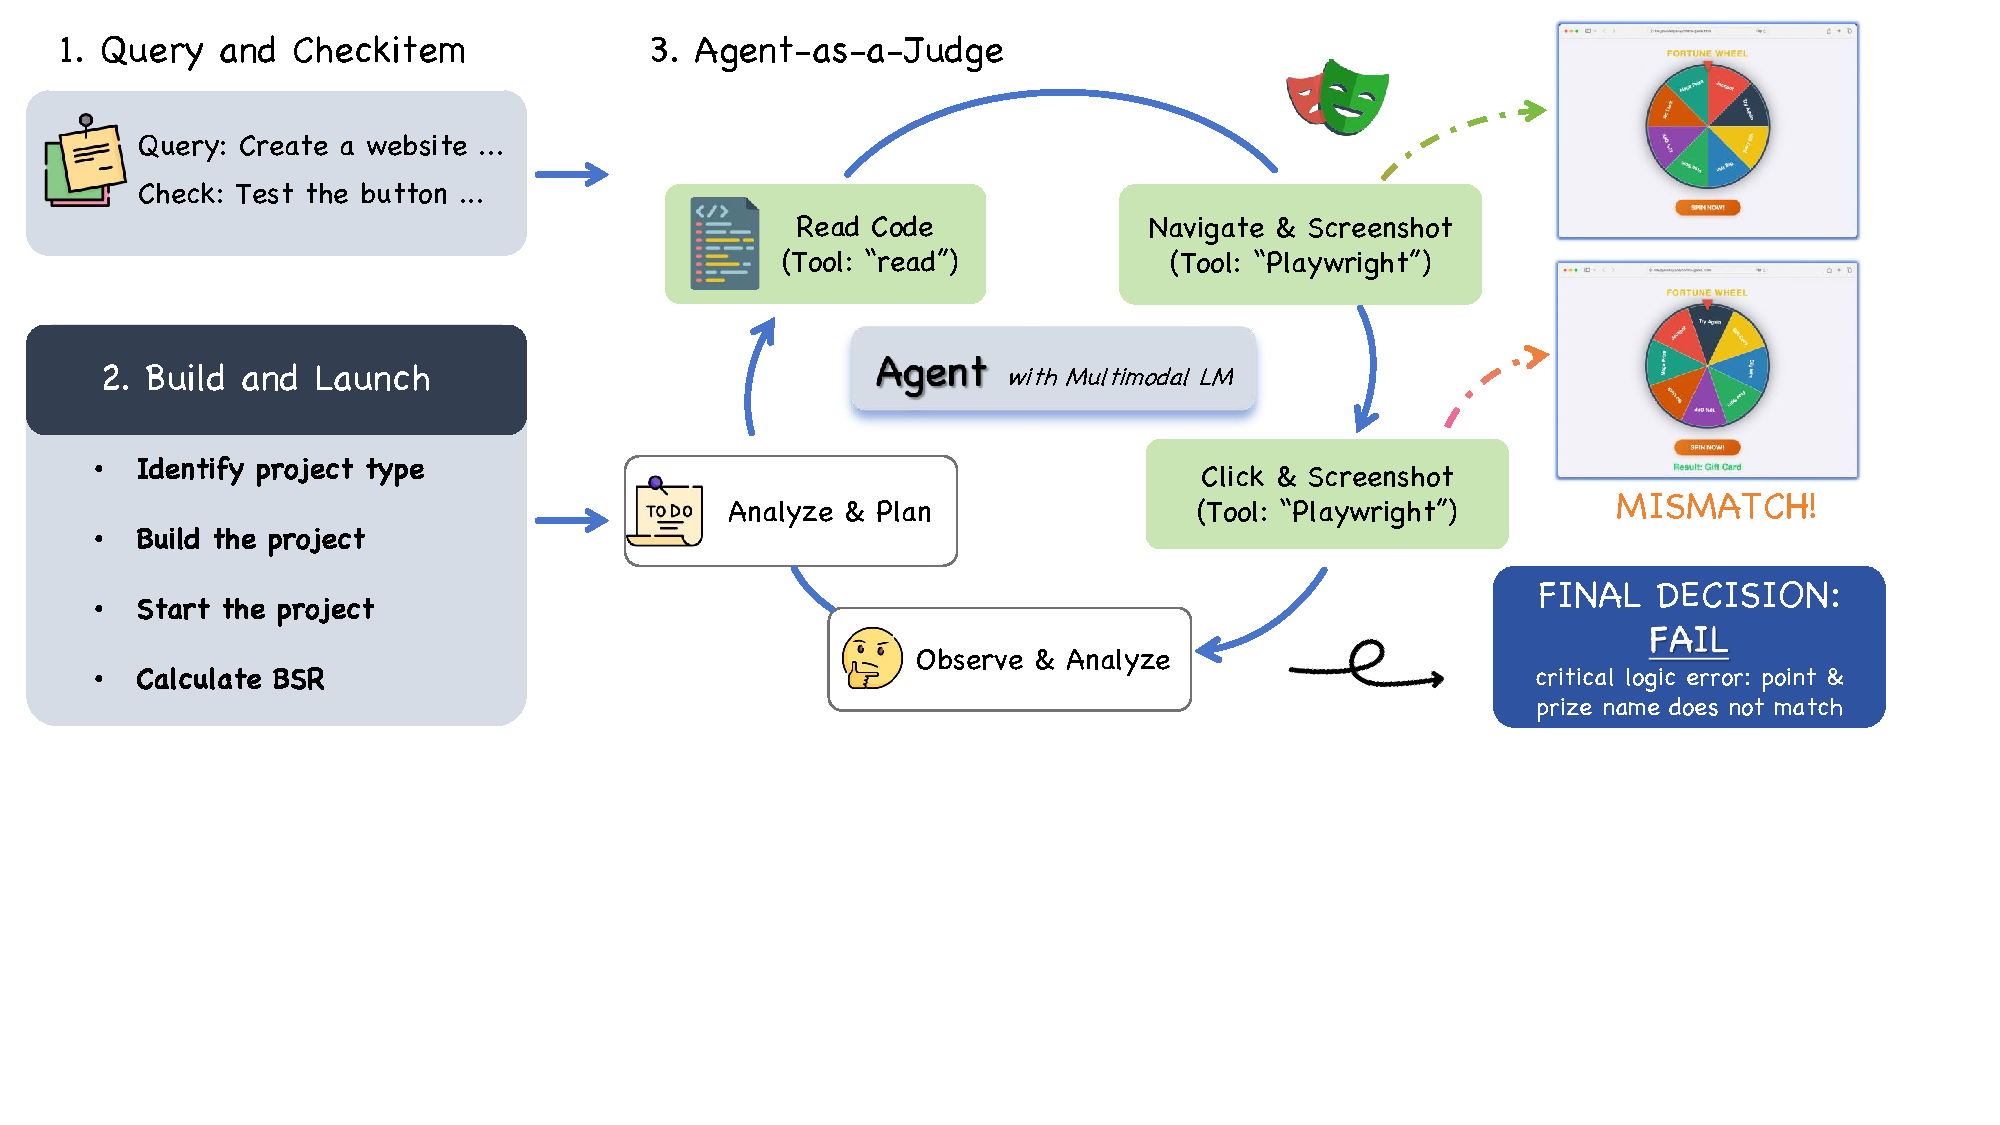
\includegraphics[width=1\linewidth]{figures/agent-as-judge.pdf}
    \vspace{-25mm}
    \caption{Agent-as-a-Judge 评测流程。每个生成的前端项目先构建以验证静态正确性。构建成功后，再由自治 Judge Agent 进行交互式测试，判定每个检查项的功能正确性。}
    \label{fig:agent-as-judge}
\end{figure}

\paragraph{Agent-as-a-Judge。}
前端正确性天然具有视觉与交互属性——缺陷常在用户点击按钮或调整窗口时才暴露，因此静态分析与固定测试集并不充分。我们据此引入 Agent-as-a-Judge（图~\ref{fig:agent-as-judge}）：每个生成项目先在 Docker 容器中部署并构建以验证静态正确性。构建成功后，交由自治 Judge Agent（Claude Code + Claude Sonnet 4.5，配备 Playwright MCP 工具）执行闭环循环：针对每个 check-item，智能体读取源码、与实时 UI 交互（点击、键入、截图）、检查终端输出，并给出通过/失败判定。

为验证可靠性，我们沿两个维度将 Agent-as-a-Judge 判定与独立人工专家判断对比。对于\emph{点位一致性}，我们抽样 130 个 check-items，由人工专家独立打分并与智能体判定比较：两者在 94\% 条目上达成一致，分歧主要集中在主观视觉质量而非功能规格。对于\emph{排序一致性}，我们使用自动框架与人工专家同时评估 8 个前沿模型（Claude Sonnet 4.5、Claude Opus 4.5、Gemini 3 Pro、GLM-4.7、DeepSeek-V3.2 等），得到的模型排序 Spearman 相关系数为 85.7\%，说明二者强正相关。

如表~\ref{tab:cc-bench-v2} 所示，GLM-5 取得 98.0\% BSR，且在 CSR 上与 Claude Opus 4.5 竞争力接近；但三种技术栈下 ISR 仍存在明显差距，表明 GLM-5 在多数单项要求上能达标，但在整任务端到端完成上仍落后于 Claude Opus 4.5。

\subsubsection{后端评估}

后端评估衡量编码智能体在真实服务端代码库与真实工程约束下，是否能做出正确且通过测试的修改。我们整理了 85 个任务，覆盖六种语言（Python、Go、C++、Rust、Java、TypeScript），涉及搜索引擎、数据库引擎、Web 框架、AI 推理服务、知识管理系统，以及独立算法与系统编程挑战。任务类型包括功能实现、缺陷修复、回归修复与性能优化，反映了日常后端开发多样性。

为实现全自动评估，每个任务配有人工编写单元测试（每题 5--10 个），同时验证功能正确性与边界情况处理。任务按 terminal-bench 风格封装：在由项目真实构建环境初始化的 Docker 容器中运行，智能体接收描述所需改动的自然语言问题陈述。我们报告 Pass@1：仅当任务全部关联单元测试通过时判定为解决。该严格全或无标准使基准更具挑战性：GLM-5 与 Claude Opus 4.5 表现相近（表~\ref{tab:cc-bench-v2}），且均显著领先 GLM-4.7。

\subsubsection{长时程评估}

长时程评估聚焦将生产级智能体工程与单轮 vibe coding 区分开的能力：在超大代码库中导航，并执行多步开发——每一步都会重塑后续步骤上下文。我们将其拆分为两项互补任务。

\textbf{大型仓库探索。} 任何非平凡编码任务的前提，都是在大型陌生仓库中定位正确源码文件。我们在真实高 star GitHub 仓库上构建自动化基准，这些仓库包含数万文件。每个问题都使用自然、面向用户的业务语义表述，严格避免文件名、类名与函数名。此外，问题需要一到两跳逻辑推断才能从用户描述映射到真实实现——例如“生成视频唇形不同步”问题需要定位到视频生成后端中的参数调优模块。目标文件按最大化导航难度选择：至少位于三级目录深处、名称不透明难以关键词检索、功能在仓库中唯一且不重复，并位于主功能面之外。我们报告三次运行平均 Pass@1；若智能体在探索过程中成功读取目标文件则记为解决。该任务中，GLM-5 优于 Claude Opus 4.5（表~\ref{tab:cc-bench-v2}），二者均显著领先 GLM-4.7。结果表明，高效仓库探索更多依赖战略搜索能力，而非纯代码生成能力——即通过目录级推理与语义关联迭代缩小文件空间，这正是 GLM-5 在智能体工具使用轨迹训练中形成的优势。

\textbf{多步链式任务。} 主流编码基准如 SWE-bench 将评估简化为单次提交、孤立编辑，因此无法衡量智能体在增量开发中的能力（每一步都会改变后续步骤的代码库状态）。为此，我们从高质量仓库中挖掘已合并 PR，并通过以下流程构建长时程基准任务链：

\begin{enumerate}[leftmargin=1.5em,itemsep=2pt]
    \item \textbf{PR 过滤。} 仅保留包含测试、提交数 3--15 且为线性（非 merge）历史的已合并 PR。
    \item \textbf{语义分组。} 由 LLM 为相邻提交两两打语义相关分；再用动态规划求解最优分组，在保持提交顺序前提下最大化组内语义一致性。
    \item \textbf{补丁分流。} 将每个任务累计 diff 切分为三类：\emph{golden patch}（智能体必须产出的核心代码）、\emph{test patch}（验证测试）与 \emph{auto-apply patch}（自动应用的配置与夹具）。
    \item \textbf{问题描述生成。} 由 LLM 基于补丁与提交信息生成每个任务的自然语言问题描述。
    \item \textbf{任务分类。} 自动分类任务（feature / bug-fix / refactor / test / config），并沿三条轴评估：错误消除、关键路径准确性与测试通过。
    \item \textbf{环境验证。} 构建 Docker 环境并应用 golden patch，验证整条任务链零回归。
\end{enumerate}

给定长度为 $K$ 的任务链，智能体从 base commit 起按序执行：完成第 $k$ 个任务后提交改动，再应用第 $k{+}1$ 个任务的 auto-apply patch，代码库状态因此累积演化。评估会逐个检查提交，并在运行完整测试套件前累计应用任务 $1$ 至 $k$ 的 test patch，从而同时捕获当前任务失败与早期任务回归。我们报告单任务 Pass@1。该链式、状态递归设计直接评估了单提交基准无法覆盖的长程上下文追踪、规划与增量开发能力。表~\ref{tab:cc-bench-v2} 显示，GLM-5 相比 GLM-4.7 显著提升，但与 Claude Opus 4.5 仍有明显差距。原因在于错误会沿任务链累积：某一步的次优编辑可能在后续任务中隐性破坏测试。缩小该差距需要在长上下文一致性与长时程自我纠错方面取得进展，这也是我们当前持续研究重点。


\subsubsection{演化 SWE 任务评估}
我们在 SWE-rebench~\cite{badertdinov2025swe} 上评估，因为 SWE-bench Verified 是静态公开人工验证测试集，且已发布超过 2 年。相比之下，SWE-rebench 基于自动化流水线持续挖掘新的真实 GitHub issue 修复任务，可进行去污染、时间稳健评估，更能衡量对新软件工程问题的泛化能力，而非静态基准上的表现。表~\ref{table:swe_rebench} 展示了 GLM-5 在 SWE-rebench 上的官方结果，我们观察到 GLM-5 能够有效泛化到新的 SWE 问题。


\begin{table}[t]
\centering
\caption{SWE-rebench（2026 年 1 月）表现。}
\begin{tabular}{lccc}
\toprule
Model & Resolved Rate (\%) & Resolved Rate SEM ($\pm$, \%) & Pass@5 (\%) \\
\midrule
Claude Opus 4.6 & 52.9\% & 1.06\% & 70.8\% \\
GPT-5.2 (xhigh) & 51.7\% & 1.21\% & 58.3\% \\
Claude Sonnet 4.5 & 47.1\% & 1.69\% & 60.4\% \\
Gemini 3 Pro & 46.7\% & 2.04\% & 58.3\% \\
Claude Opus 4.5 & 43.8\% & 0.93\% & 58.3\% \\
GLM-5 & 42.1\% & 1.21\% & 50.0\% \\
GLM-4.7 & 41.3\% & 2.12\% & 56.3\% \\
% MiniMax M2.5 & 39.6\% & 0.66\% & 56.3\% \\
Kimi K2.5 & 37.9\% & 1.21\% & 50.0\% \\
\bottomrule
\end{tabular}
\label{table:swe_rebench}
\end{table}


\subsection{真实世界通用能力评估}

\begin{figure}
    \centering
    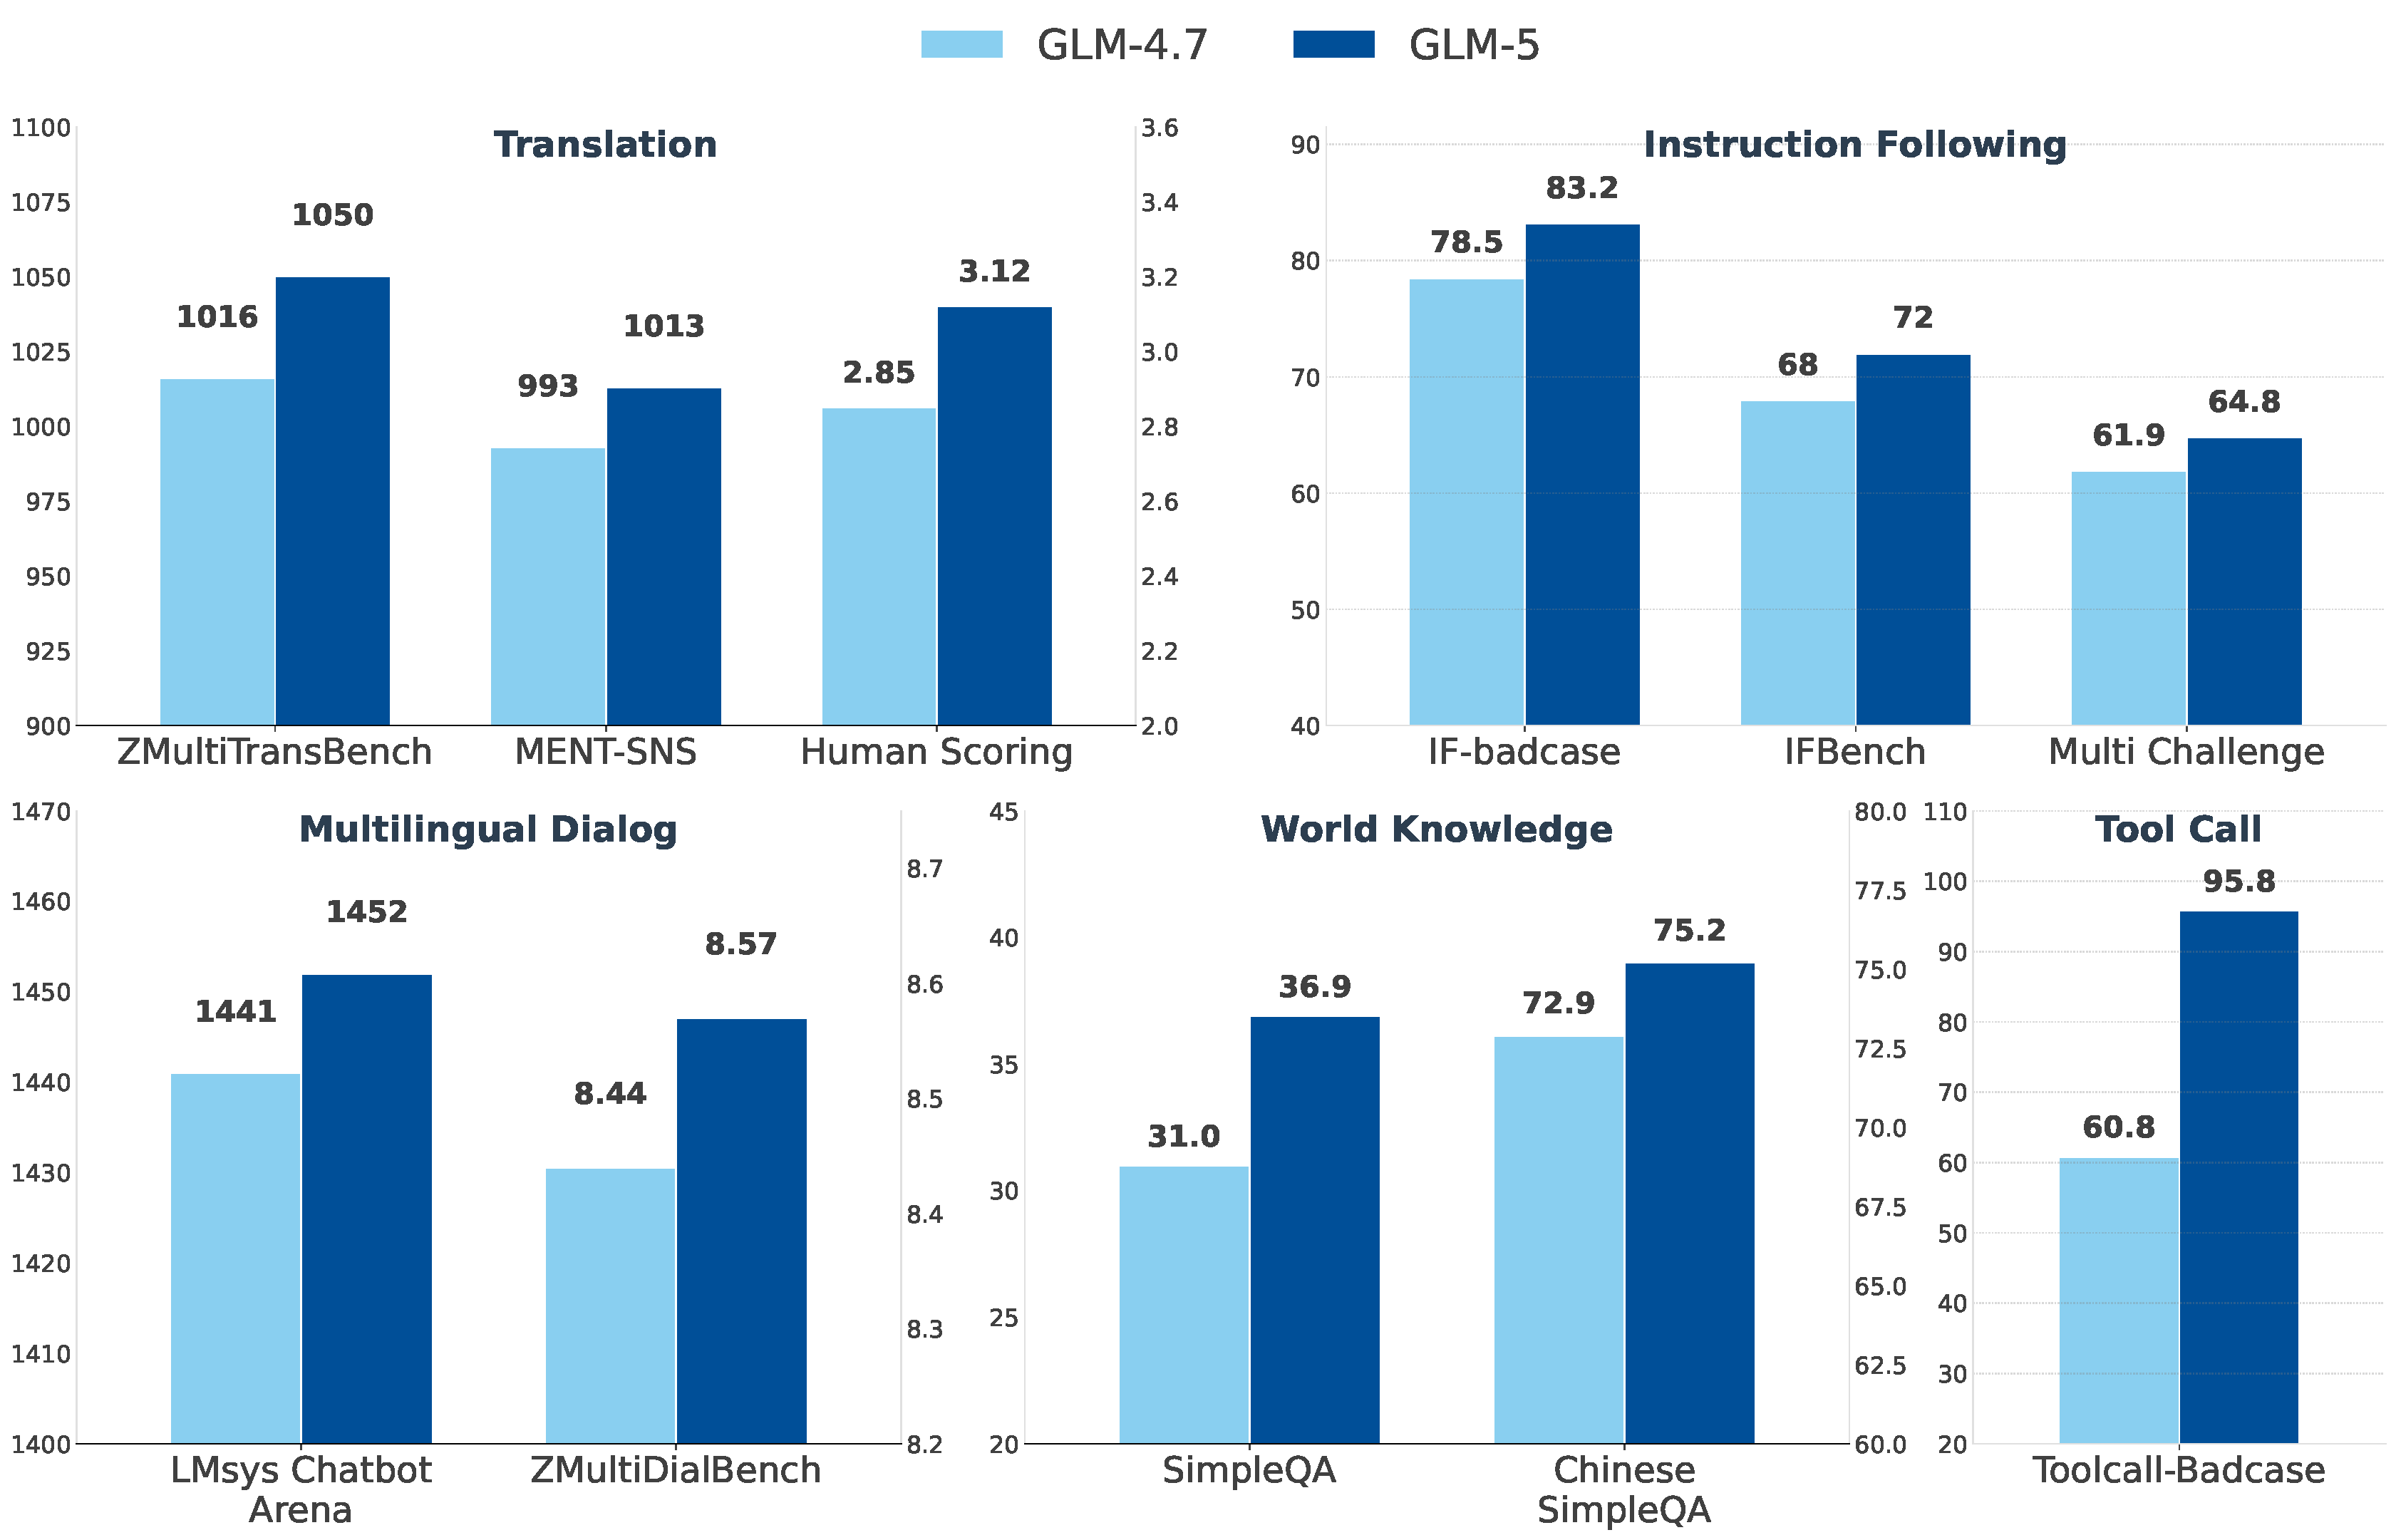
\includegraphics[width=1\linewidth]{figures/glm5_realscene_comparison.pdf}
    \caption{GLM-4.7 与 GLM-5 在五类真实世界通用能力上的性能对比。}
    \label{fig:glm5_realscene}
\end{figure}

尽管标准学术基准能提供有用信号，但它们无法完整反映模型在真实场景中的使用方式。基于这一差距，我们构建了来自高频真实用户交互模式的通用能力评估，包含 {机器翻译、多语对话、指令遵循、世界知识与工具调用}。

不同于传统“基准中心”评测，我们的目标是衡量可直接转化为用户可感知体验提升的改进。针对每项能力，我们结合内部人工评测、内部自动评测、外部人工评测与外部自动基准，兼顾诊断粒度与跨模型可比性。在使用外部基准时，我们优先选择更贴近真实交互模式的数据集，而非分布过窄的人造测试。

图~\ref{fig:glm5_realscene} 展示了 GLM-5 与 GLM-4.7 在五类真实能力上的对比。GLM-5 在机器翻译、多语对话、指令遵循、世界知识与工具调用各维度均有一致提升。


各能力的详细评测协议与数据集说明如下。 % in the following subsections.

\subsubsection{机器翻译}

\paragraph{ZMultiTransBench。}
该内部数据集包含 1,220 条样本，来自自采高频翻译场景，覆盖 7 个语言对：Zh to Es（\(300\)）、Ru（\(250\)）、Fr（\(220\)）、Ko（\(200\)）、Ja（\(150\)）、Ar（\(50\)）和 De（\(50\)）。全部样本由受过翻译学系统训练的研究生完成整理、翻译与独立核验。数据集强调自然使用语境，而非人工构造测试样例。评估采用与固定基线回复的成对比较，由基于 GPT-4.1 的自动评估器根据语义忠实度、流畅性与整体翻译质量进行判定。


\paragraph{MENT-SNS。}
为进一步评估在语言学挑战场景下的鲁棒性，我们采用 MENT \citep{tian2026ment} 的源句，包含 \(753\) 条英中句对，覆盖四个领域：社交网络（SNS）、跨文化、诗歌与文学。
这些领域用于压力测试复杂语言现象下的翻译能力，包括俚语、谐音双关、习语表达、历史典故与隐喻语言。与 ZMultiTransBench 一样，全部样本均由受过专业训练的研究生整理与核验。
评估同样采用与基线回复的成对比较协议，并使用 GPT-4.1 作为自动 judge。

\subsubsection{多语对话}
\paragraph{LMArena。}
我们报告来自 LMArena\footnote{https://arena.ai/leaderboard/text}
 的 Elo 评分，该评分来源于大规模社区提交的成对比较。该评分反映了开放式对话场景中的相对模型偏好，并提供了外部对话性能信号。

\paragraph{ZMultiDialBench。}
除公开榜单外，我们还在内部多语对话基准 ZMultiDialBench 上进行人工评测。该数据集包含 141 条精心整理样本，覆盖多类对话类型。样本来源于多国母语标注者贡献的高质量对话数据，以及线上用户反馈的高难失败案例。
人工标注者依据分类型标准评测规范，对匿名化模型回复进行 1–10 分点位打分。

\subsubsection{指令遵循}
\paragraph{IF-Badcase。} IF-Badcase 是由生产环境真实用户上报的指令遵循\textbf{失败样例}构建的内部基准。该数据集用于评估对真实多约束指令的严格遵循，重点关注流程准确性、逻辑一致性与严格格式要求。
评估采用细化 checklist 协议，验证模型是否满足显式约束，包括步骤顺序、规则条件与结构规范。全部样本经人工专家多轮标注、复核与迭代过滤，最终形成 450 条高质量测试样本。

\paragraph{IF-Bench~\citep{ifbench}.} IF-Bench 评估 LLM 对复杂客观约束（如特定格式规则、长度限制、内容限制）的遵循能力。该基准提供对精确指令遵循能力的量化评估，聚焦可验证合规性而非开放式生成质量。

\paragraph{MultiChallenge~\citep{multichallenge}.} MultiChallenge 通过真实多轮对话场景评测 LLM。其目标是检验复杂交互中准确指令遵循、上下文分配与上下文内推理能力。


\subsubsection{世界知识}

\paragraph{SimpleQA~\citep{simpleQA}.} SimpleQA 通过具有唯一明确答案的高难问题衡量短答案事实性。该基准通过将回复分类为正确、错误或未作答来评估模型校准能力，强调准确性而非生成长度。

\paragraph{Chinese SimpleQA~\citep{chinesesimpleQA}.} 该基准将 SimpleQA 方法适配到中文语境，覆盖六大领域与 99 个子主题。它使用高质量、静态、短答案问题并支持可靠自动评分，用于评估 LLM 的知识准确性。

\subsubsection{工具调用}
\paragraph{ToolCall-Badcase。} ToolCall-Badcase 是由生产环境用户上报的工具调用\textbf{失败样例}构建的内部基准。每个样本都配有可验证真值工具调用，可对工具选择与参数正确性进行客观评估。
评估检查模型是否（1）调用正确工具，以及（2）提供结构正确且语义准确的参数。
全部样本均经过多轮复核、改写与验证，以消除歧义并确保可评测性。最终数据集包含 200 条高质量测试样例，反映真实工具调用能力。
